%% This is file `elsarticle-template-1-num.tex',
%%
%% Copyright 2009 Elsevier Ltd
%%
%% This file is part of the 'Elsarticle Bundle'.
%% ---------------------------------------------
%%
%% It may be distributed under the conditions of the LaTeX Project Public
%% License, either version 1.2 of this license or (at your option) any
%% later version.  The latest version of this license is in
%%    http://www.latex-project.org/lppl.txt
%% and version 1.2 or later is part of all distributions of LaTeX
%% version 1999/12/01 or later.
%%
%% Template article for Elsevier's document class `elsarticle'
%% with numbered style bibliographic references
%%
%% $Id: elsarticle-template-1-num.tex 149 2009-10-08 05:01:15Z rishi $
%% $URL: http://lenova.river-valley.com/svn/elsbst/trunk/elsarticle-template-1-num.tex $
%%
\documentclass[preprint,12pt]{elsarticle}
\usepackage[utf8]{inputenc}
\usepackage[T1]{fontenc}
\usepackage{lmodern}
\usepackage{graphicx}
\usepackage[figurename=Fig.,labelfont=bf,labelsep=period]{caption}
\usepackage{subcaption}
\usepackage{amsmath}
\usepackage{lscape}
\usepackage{makecell}
\usepackage{slashbox}
\usepackage{array, makecell} %

%\usepackage{hyperref}

%\usepackage{amsfonts}
%\usepackage{amssymb}
%\usepackage{amsbsy}
\usepackage{newtxtext,newtxmath}
\usepackage[colorlinks=true,citecolor=red,linkcolor=black]{hyperref}
%% Use the option review to obtain double line spacing
%% \documentclass[preprint,review,12pt]{elsarticle}

%% Use the options 1p,twocolumn; 3p; 3p,twocolumn; 5p; or 5p,twocolumn
%% for a journal layout:
%% \documentclass[final,1p,times]{elsarticle}
%% \documentclass[final,1p,times,twocolumn]{elsarticle}
%% \documentclass[final,3p,times]{elsarticle}
%% \documentclass[final,3p,times,twocolumn]{elsarticle}
%% \documentclass[final,5p,times]{elsarticle}
%% \documentclass[final,5p,times,twocolumn]{elsarticle}

%% The graphicx package provides the includegraphics command.

%% The amssymb package provides various useful mathematical symbols
\usepackage{amssymb}
%% The amsthm package provides extended theorem environments
%% \usepackage{amsthm}

%% The lineno packages adds line numbers. Start line numbering with
%% \begin{linenumbers}, end it with \end{linenumbers}. Or switch it on
%% for the whole article with \linenumbers after \end{frontmatter}.
\usepackage{lineno}

%% natbib.sty is loaded by default. However, natbib options can be
%% provided with \biboptions{...} command. Following options are
%% valid:

%%   round  -  round parentheses are used (default)
%%   square -  square brackets are used   [option]
%%   curly  -  curly braces are used      {option}
%%   angle  -  angle brackets are used    <option>
%%   semicolon  -  multiple citations separated by semi-colon
%%   colon  - same as semicolon, an earlier confusion
%%   comma  -  separated by comma
%%   numbers-  selects numerical citations
%%   super  -  numerical citations as superscripts
%%   sort   -  sorts multiple citations according to order in ref. list
%%   sort&compress   -  like sort, but also compresses numerical citations
%%   compress - compresses without sorting
%%
%% \biboptions{comma,round}

% \biboptions{}

\journal{Journal Name}

\begin{document}

\begin{frontmatter}

%% Title, authors and addresses

\title{Knowledge-Base Data Integration of Urban Sustainable Indicators}

%% use the tnoteref command within \title for footnotes;
%% use the tnotetext command for the associated footnote;
%% use the fnref command within \author or \address for footnotes;
%% use the fntext command for the associated footnote;
%% use the corref command within \author for corresponding author footnotes;
%% use the cortext command for the associated footnote;
%% use the ead command for the email address,
%% and the form \ead[url] for the home page:
%%
%% \title{Title\tnoteref{label1}}
%% \tnotetext[label1]{}
%% \author{Name\corref{cor1}\fnref{label2}}
%% \ead{email address}
%% \ead[url]{home page}
%% \fntext[label2]{}
%% \cortext[cor1]{}
%% \address{Address\fnref{label3}}
%% \fntext[label3]{}


%% use optional labels to link authors explicitly to addresses:
%% \author[label1,label2]{<author name>}
%% \address[label1]{<address>}
%% \address[label2]{<address>}

\author{Emanuele Massaro, Claudia Binder}
\address{HERUS Lab, EPFL, Switzerland}
\author{Aristide Athanassiadis}
\address{Circular Economy and Urban Metabolism, Université Libre de Bruxelles, Belgium, Belgium}
\author{Achilleas Psyllidis}
\address{Web Information Systems, Delft University, Netherlands}

\begin{abstract}
%% Text of abstract
Before submission
\end{abstract}

\begin{keyword}
\\ Sustainability Assessment \sep Knowledge Base \sep Ontology \sep Urban Indicators
%% keywords here, in the form: keyword \sep keyword

%% MSC codes here, in the form: \MSC code \sep code
%% or \MSC[2008] code \sep code (2000 is the default)

\end{keyword}

\end{frontmatter}

%%
%% Start line numbering here if you want
%%
\linenumbers

%% main text
\section{Introduction}
The complexity, structure, and dynamics of cities and urban systems are multi-scalar in nature. In a similar way, data and information about how cities perform involve a range of spatial scales, from a disaggregate (e.g. individual activities, events at specific locations etc.) to an aggregate (e.g. neighborhoods, census tracts, entire cities as single entities) level. This has an impact on how we measure, evaluate, and understand problems facing contemporary cities. Examples of the latter include the population growth or, in some occasions, shrinkage in urban areas, the use of energy resources to sustain city populations and urban infrastructure, as well as the circulation of goods and people across the urban fabric, to name a few. In response to the aforementioned problems, policies about modern-day cities call for increased sustainability, resilience, and circularity of materials and resources to improve the overall quality of life. Despite the importance of these aspects in assuring a better well-being for urban populations, the lack of coherent and common definitions results in ambiguous interpretations and, further, makes their quantitative and qualitative evaluation rather cumbersome. In this chapter, we focus specifically on the aspect of urban sustainability.

In better understanding the factors that contribute to a sustainable urban environment, a wealth of indicators, structured in the form of standards (e.g. ISO, OECD, SDG Index etc.), have been developed and proposed over the past decades. These standards aim to pull apart the concept of sustainability and take different approaches to understanding the dimensions that contribute to sustainable cities and urban systems. The indicators comprising the standards are primarily the result of empirical data, derived from a variety of sources. Despite the multiplicity of existing indicators, there is currently a lack of consensus among the various standards. For instance, similar indicators are described using different terms or similar terms are used to refer to different indicators.
% (add an example)
The current lack of consensus among the various standards poses challenges to the measurement, evaluation, and comparison of urban sustainability performance across cities.

An approach to fostering the interoperability among the different urban sustainability standards could involve the use of ontologies \cite{psyllidis2016dis,psyllidis2015}. Ontologies play a pivotal role in semantic integration and data interoperability, by accounting for shared vocabularies and formal definitions of domain concepts and their interrelationships. These concepts represent real-world entities, which are expressed in a machine-processable format, meaning that they can be further interpreted by computing systems. Despite the different knowledge representation languages used (e.g. OWL, RDFS etc.), ontology concepts are most frequently represented as classes. These are subsequently organized into hierarchies or taxonomies, connecting the different concepts together through explicitly defined relationships. Other essential features of ontologies include attributes, which enrich concepts with data types (e.g. integers, strings, Booleans etc.) and values, as well as axioms, which constitute logical statements (e.g. a class is kind of another class, or a class is different from another class etc.) enriching the knowledge about the domain in question.  At the data level, ontologies are further characterized by instances — also referred to as individuals — which constitute specific objects belonging to more generic classes (e.g. a train station is an instance of a generic class representing all types of buildings). Being built on these components, ontologies constitute prominent repositories for sharing, interpreting, and reusing knowledge about a domain.

This chapter introduces an ontology-driven framework for the semantic interoperability of urban sustainability standards. It presents and describes a formal representation of knowledge about sustainability indicators and their interrelationships, through the development of a domain ontology. Given the dynamic redefinition of sustainability indicators, we demonstrate how the proposed ontology-driven framework offers a flexible approach to documenting and semantically representing urban sustainability standards, as opposed to fixed data schemata.  To increase the adaptability and reuse, as well as to facilitate its continuous redevelopment, we make the developed ontology available online, through a dedicated web portal.

The remainder of this chapter is organized as follows. First, we present a set of prevalent standards and their corresponding indicators, used in urban sustainability studies. Next, we introduce the proposed ontology-driven framework and describe the ontology for urban sustainability. We specifically focus on how the ontology allows for semantic linkages among the indicators included in the numerous existing standards. Finally, we discuss the limitations of our framework, summarize the conclusions, and describe future lines of research.
 \begin{table}[t!]
 \caption{Total number of indicators and source of information for the different frameworks.}
     \begin{tabular}{ | p{2.3cm}| p{1cm} |  p{9.3cm} |}
  \hline
  Name & N & Source\\
   \hline 
   \hline
  OECD & 41 & \url{https://stats.oecd.org/} \\
   \hline
  ISO 37120 & 133 & \url{http://www.dataforcities.org/wccd/} \\
     \hline
  SDG  & 48 & \url{http://unsdsn.org/resources/publications/us-cities-sdg-index/} \\
       \hline
   CI  & 34 & \url{https://www.bfs.admin.ch/bfs/en/home/statistics/sustainable-development.html} \\
       \hline
 UMI  & 83 & Reference \cite{kennedy2014developing} \\
  \hline  
 \label{tab:numberIndicators}
\end{tabular}
 \end{table}
 
\section{Urban Indicators of sustainability}
\label{sec:UIS}
Urban sustainability indicators are a key element to assess the sustainability of cities, define quantitative objectives and monitor the progress towards them, as well as to develop communication between different stakeholders \cite{SHEN201117}. In fact, a number of researchers, private companies or consultants as well as international administrations have worked on developing sustainability indicators for specific or a group of cities. Yet, at this stage there is no consensus on urban sustainability indicators that fuels unconsolidated and difficultly comparable findings \cite{kahn2007green}. The lack of consensus on the choice of indicators is very closely related to the fact, that there is no common definition as to what urban sustainability or a sustainable city is \cite{alberti1996measuring}. Due to the numerous and complex ways cities are impacting and are impacted by the environment both locally and globally, a unique definition and sustainability indicators appear to be intangible.

This subsection will present a number of indicators framework that focus on urban sustainability. The motivation to build the indicator frameworks, the similarities and differences amongst them as well as how certain sustainability aspects are considered by them will be discussed in this Chapter. More specifically, the indicators framework, summarized in Table 1, that will be presented in this part are the following:
\begin{enumerate}
\item OECD: the OECD indicators;
\item ISO 37120: ISO standard 37120 on the sustainable development of communities (International Organization for Standardization (ISO) 2014);
\item SDG: U.S. Cities SDG Index \cite{prakash2017us};
\item CI: Cercle indicators from the Swiss federal office of statistics;
\item UMI: the urban metabolism indicators.
\end{enumerate}



\subsection{ISO standard 37120}
The ISO standard 37120 for sustainable development of communities provides a standardised set of indicators of city services and quality of life that is claimed to be “comparable over time … [and] across cities”. The transposable character of the indicator framework facilitates cities to learn one from another when comparing their data and local initiatives. The standard puts together more than 100 indicators around three main types of indicators. Profile indicators which provides more context about a city and enables its comparison with others. These include generic information about demography, economy, climate, etc. Core indicators, which candidate cities need to provide data in order to receive a certification and finally supporting indicators which are highly recommended indicators but not mandatory. Core and supporting indicators are classified in 17 broad themes including: economy, education, energy, environment, finance, fire and emergency response, governance, health, recreation, safety, shelter, solid waste, telecommunication and innovation, transportation, urban planning, wastewater, water and sanitation. As visible, the indicator framework covers a wide range of urban aspects which are not necessarily linked to urban sustainability, per se, but on the capacity of a city to provide some specific services to its inhabitants.

\subsection{The Cercle Indicators}
The Cercle Indicators are sustainability indicators for Swiss Cantons and Municipalities developed by the Swiss Federal office for Territorial Development (Office fédérale du développement territorial \cite{meier2005indicators}. This indicator set was developed to benchmark the evolution Swiss cities towards sustainability as well as identify where they should focus their efforts to accelerate this transition. Urban sustainability is considered under its three dimensions, namely environment, economy and society. Within each dimension, 11 to 12 themes are considered (more details about the themes are provided at Table 1) and one central indicator is used to represent these themes. Using the Cercle Indicators helps decision makers to develop and implement action plans as well as communicate more easily on urban sustainability. Yet, as the indicators remain quite vague, they don’t enable to assess specific policies or projects. This indicator set is structured along the traditional elements of sustainability and attempts to enable them on urban territories. Yet, it does not necessary takes into account the specificity and context of urban systems.


\subsection{OECD regional and metropolitan databases}
The Organisation for Economic Co-operation and Development has develop two statistical databases that provide comparable indicators for about 2000 regions and 281 OECD metropolitan areas (urban areas with 500 000 or more inhabitants). The 41 indicators about metropolitan areas cover economic (GDP and patent activities), geographic and administrative forms, environmental, social (income and inequality), labour market and demographic indicators.

\subsection{Urban metabolism indicators}
Urban metabolism is scientific community comparing the functioning of cities to a living organism \cite{kennedy2015energy}. While there are different disciplinary vantage points behind the community, an essential element of urban metabolism is the assessment of material, energy water and other flows entering and exiting urban systems. A number of studies have characterized the flows of cities across the globe, yet data availability and accuracy is a pervasive challenge \cite{athanassiadis2017towards,barles2009urban,athanassiadis2017exploring,niza2009urban,hoekman2017cape,voskamp2017enhanced}. Depending on data availability authors choose different type of accounting methods, and therefore indicators and data to characterize the metabolism of cities. A number of cases have used Economy-Wide Material Flow Accounting, which was initially developed for nation-wide economies, due to its set accounting method and enabling comparability. Some authors have brought in modifications to the existing method to better encompass what happens at an urban level (Voskamp et al. 2016; Barles 2009). Other researchers have simply compiled data from metabolic flows with no particular methodological depending on data availability. The inconsistency of the indicators used by researchers to measure the metabolic flows represents one of the main challenges of the community as the results is a juxtaposition of assessments that do not enable to develop a robust theoretical and methodological framework. Kennedy et al. \cite{kennedy2014developing} proposed an indicator set for urban metabolism that was later applied to 27 megacities, which is the largest sample of comparable cities from a metabolic perspective \cite{kennedy2015energy}.
The indicator list proposed, which is a smaller and more pragmatic set of indicators from the ones proposed by (Kennedy and Hoornweg 2012), is divided in four layers of information that provide quantitative and qualitative information about the metabolism of megacities. The first layer covers the definition of a megacity, or in other words the spatial and administrative delimitation of the city as well as information on population and GDP. The second layer presents biophysical characteristics of megacities including climatic and building floor area details. The third layer focuses on the characterisation of metabolic flows per se, meaning the quantification of energy, water, waste, materials flows and of the material stock. The final layer provides qualitative information about the utilities that circulate and metabolise the flows quantified in the previous layers.

The main objective of urban metabolism indicators is to help understand the mechanisms that are behind urban resource use and pollution emissions in order to develop mitigation strategies. From that perspective, this set of indicators is focusing on the environmental aspect of urban sustainability offering an academic perspective.

\subsection{U.S. Cities SDG Index}
This indicator set presented here is derived from the 17 Sustainable Development Goals (SDG) developed by the United nations applied to U.S. cities. In 2015, the SDGs replaced the Millennium Development Goals (and its 60 indicators) and included goals amongst others about poverty, hunger, health, or sustainable cities and communities. Based on these goals, an SDG index with 79 indicators and using data from international organisations (such as the World Bank, Food and Agriculture Organisation, etc.) was developed to track the progress or performance of countries on the SDGs \cite{sachs2016sdg}. The U.S. Cities SDG Index, transposes the above mentioned Global SDG Index to 100 most populous cities of the United States of America or more specifically metropolitan statistical areas as they offer a better data availability. This urban index consists of 49 indicators and its main objectives are to provide a database to monitor sustainable development in American cities, to better understand where U.S. cities stand on SDG implementation as well as identify potential actions to accelerate this implementation, and finally identify data gaps that hinder cities to monitor the implementation of SDGs. Most of the data required to cover the 49 indicators of the index are provided by the American Community Survey, yet they do not always reflect the full extent of each goal. In addition, as one of the 17 goals is specifically focusing on cities and communities (goal 11), the question is raised as to whether the rest of the goals should be enquired or more indicators should be included for SDG 11. As per the Cercle Indicators, the U.S. Cities SDG Index covers a wide array of urban sustainability aspects but remains quite superficial thus not necessarily enabling the development of mitigation action plans.




 

% \begin{landscape}
% \begin{center}
%     \begin{tabular}{ | p{3cm} | p{3.5cm} | p{3.5cm} |  p{
%     3.5cm} |  p{3.5cm} |  p{3.5cm} |}
%     \hline
%     & ISO 37120 & \makecell{Cercle \\ Indicators} & OECD & SDG & \makecell{Urban \\ Metabolism} \\ \hline
%     \textbf{\makecell{Motivation \\ Objectives}} & \small{Transposable
% City services and quality of life}
%  &  &  & \small{Measure progress towards SDGs} & \small{Measure the flows of resource use and pollution emission entering and exiting cities} \\   \hline

%     \textbf{\makecell{Number of \\ indicators}} & 
% 133
% &
% 35
% &
% 41
% &
% 17
% &
% 90
% \\   \hline
 
%     \textbf{\makecell{How indicators \\ are classified?}} & 
%     \small{Themes (but also divided in profile, core and supporting indicators)}
%  & \small{Three dimensions (environment, economy, society) and within themes} & \small{Themes and indicators are mentioned as variables} & \small{Goals} & \small{Layers} \\   \hline
 
 
%     \textbf{\makecell{What are the \\ different classes \\ included?}} & 
%     \small{Economy, education, energy, environment, finance, fire and emergency response, governance, health, recreation, safety, shelter, solid waste, telecommunication and innovation, transportation, urban planning, wastewater, water and sanitation.)}
%  & \small{\textbf{Environment} (biodiversity, nature and landscape, quality of energy, energy consumption, climate, air quality, etc).
% \textbf{Economy} (income, life costs, job market, investments, etc).
% \textbf{Society} (housing quality, mobility, health, security, income distribution, etc
% } & \small{Themes and indicators are mentioned as variables} &  & \\   \hline
 
%     \textbf{\makecell{What parts of \\ urban \\ sustainability \\ are covered?}} & 
    
%  &  &  &  &  \small{Environmental flows and economic parts of sustainability, nor a link to the impact of these flows to the environment).} \\   \hline

%     \textbf{\makecell{Examples}} & 
    
%  &  &  &  &  \small{Water consumption, share of electricity sources, net import of cement, etc.} \\   \hline


%     \end{tabular}
% \end{center}

% \end{landscape}


\section{Ontology Development}
In this section we describe the methods and the phases we used in order to aggregate and combine different sustainable indicators extracted from the different 5 frameworks in forms of an \emph{Ontology}.

\subsection{Objectives of an Ontology}
An ontology defines a common vocabulary for researchers who need to share information in a domain. It includes machine-interpretable definitions of basic concepts in the domain and relations among them.

Why would someone want to develop an ontology? Some of the reasons are:
\begin{itemize}
\item To share common understanding of the structure of information among people or software agents
\item To enable reuse of domain knowledge
\item To make domain assumptions explicit
\item To separate domain knowledge from the operational knowledge
\item To analyze domain knowledge
\end{itemize}

\emph{Sharing common understanding of the structure of information among people or software agents}  is one of the more common goals in developing ontologies \cite{gruber1995toward}. For example, suppose several different Web sites contain medical information or provide medical e-commerce services. If these Web sites share and publish the same underlying ontology of the terms they all use, then computer agents can extract and aggregate information from these different sites. The agents can use this aggregated information to answer user queries or as input data to other applications.

\emph{Enabling reuse of domain knowledge} was one of the driving forces behind recent surge in ontology research. For example, models for many different domains need to represent the notion of time. This representation includes the notions of time intervals, points in time, relative measures of time, and so on. If one group of researchers develops such an ontology in detail, others can simply reuse it for their domains. Additionally, if we need to build a large ontology, we can integrate several existing ontologies describing portions of the large domain. We can also reuse a general ontology, such as the UNSPSC ontology, and extend it to describe our domain of interest.

\emph{Making explicit domain assumptions} underlying an implementation makes it possible to change these assumptions easily if our knowledge about the domain changes. Hard-coding assumptions about the world in programming-language code makes these assumptions not only hard to find and understand but also hard to change, in particular for someone without programming expertise. In addition, explicit specifications of domain knowledge are useful for new users who must learn what terms in the domain mean. 

\emph{Separating the domain knowledge from the operational knowledge} is another common use of ontologies. We can describe a task of configuring a product from its components according to a required specification and implement a program that does this configuration independent of the products and components themselves \cite{mcguinness1998usability}. We can then develop an ontology of PC-components and characteristics and apply the algorithm to configure made-to-order PCs. We can also use the same algorithm to configure elevators if we “feed” an elevator component ontology to it.

\emph{Analyzing domain knowledge} is possible once a declarative specification of the terms is available.  Formal analysis of terms is extremely valuable when both attempting to reuse existing ontologies and extending them \cite{mcguinness2000chimaera}.

Often an ontology of the domain is not a goal in itself. Developing an ontology is akin to defining a set of data and their structure for other programs to use. Problem-solving methods, domain-independent applications, and software agents use ontologies and knowledge bases built from ontologies as data. For example, in this paper we develop an ontology of wine and food and appropriate combinations of wine with meals. This ontology can then be used as a basis for some applications in a suite of restaurant-managing tools: One application could create wine suggestions for the menu of the day or answer queries of waiters and customers. Another application could analyze an inventory list of a wine cellar and suggest which wine categories to expand and which particular wines to purchase for upcoming menus or cookbooks.

The goal of this research is to i) Sharing common understanding of the structure of information among scholars and stakeholders and ii) Enabling reuse of domain knowledge and iii) Analyzing domain knowledge in the field of urban sustainability assessment. We aggregate the different sustainable indicators proposed by the 5 different frameworks described above in form of ontology by defining a hierarchical structure and links between different classes and indicators.

\subsection{What is an Ontology?}
The literature contains many definitions of an ontology; many of these contradict one another \cite{guarino2009ontology}. For the purposes of this research, we define an ontology as a formal explicit description of concepts in a domain of discourse (\textbf{classes}), properties of each concept describing various features and attributes of the concept (\textbf{properties}) and \textbf{relations} between classes and individuals. An ontology together with a set of individual instances of classes constitutes a knowledge base. 

Classes are the focus of most ontologies. Classes can be defined as an extension or an intension. According to an extensional definition, they are abstract groups, sets, or collections of objects. According to an intensional definition, they are abstract objects that are defined by values of aspects that are constraints for being member of the class. The first definition of class results in ontologies in which a class is a subclass of collection. The second definition of class results in ontologies in which collections and classes are more fundamentally different. Classes may classify individuals, other classes, or a combination of both. Some examples of classes:
\begin{itemize}
\item Person, the class of all people, or the abstract object that can be described by the criteria for being a person.
\item Vehicle, the class of all vehicles, or the abstract object that can be described by the criteria for being a vehicle. A car can be a sub-class of Vehicle.
\item Class, representing the class of all classes, or the abstract object that can be described by the criteria for being a class.
\item Thing, representing the class of all things, or the abstract object that can be described by the criteria for being a thing (and not nothing).
\end{itemize}
Importantly, a class can subsume or be subsumed by other classes; a class subsumed by another is called a \textbf{subclass} (or subtype) of the subsuming class (or supertype). For example, \emph{Air Pollution} subsumes $CO_2$ emissions, since (necessarily) anything that is a member of the latter class is a member of the former. Relationships (also known as relations) between objects in an ontology specify how objects are related to other objects. Typically a relation is of a particular type (or class) that specifies in what sense the object is related to the other object in the ontology. For example, in the ontology that contains the concept \emph{OECD} and the concept GHG (green house emissions) that might be related by a relation of type \texttt{is defined by}. The full expression of that fact then becomes in form of a semantic triple:\\
\begin{center}
GHG \texttt{is defined by} OECD \\
subject \quad  predicate \quad object
\end{center}

An important type of relation is the subsumption relation (\texttt{is-a-subclass-of}). This defines which objects are classified by which class. For example, we have already seen that the class GHG \texttt{is-a-subclass-of} Air Pollution, which in turn \texttt{is-a-subclass-of} Air. The addition of the is-a-subclass-of relationships creates a taxonomy; a tree-like structure (or, more generally, a partially ordered set) that clearly depicts how objects relate to one another. In such a structure, each object is the 'child' of a 'parent class' (Some languages restrict the is-a-subclass-of relationship to one parent for all nodes, but many do not). An example of hierarchical taxonomic hierarchy of classes and subclasses is shown in \figurename~\ref{fig:ontologyScheme}. In practical terms, developing an ontology includes:
\begin{itemize}
\item defining classes in the ontology,
\item arranging the classes in a taxonomic (subclass–superclass) hierarchy,
\item defining slots and describing allowed values for these slots,
\item filling in the values for slots for instances.
\end{itemize}
\begin{figure}[htb!]
\centering
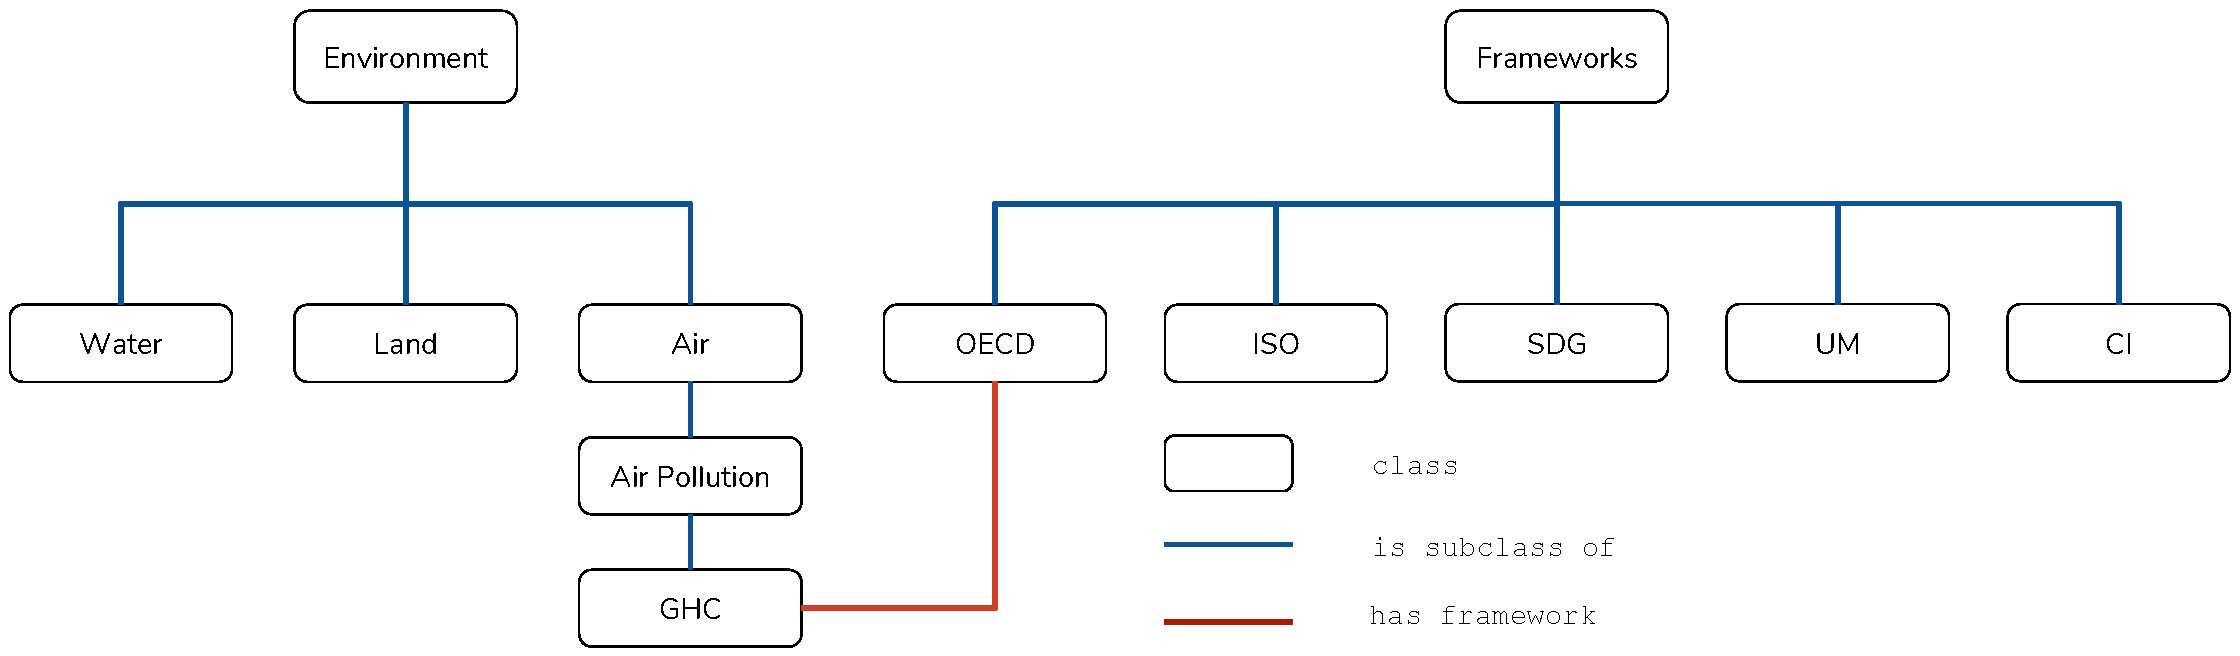
\includegraphics[width=1\textwidth]{figures/ontology2.pdf}
\caption{Example of an ontology scheme where white boxes are classes, blue links are sub-class relationships and the red links are framework properties. In this ontology we have two super classes: Environment and Frameworks with different subclasses. The indicator GHG which represents Green House Emission is a subclass of Air Pollution and has as a property the fact that is defined by the framework OECD. }
\label{fig:ontologyScheme}
\end{figure}

\subsection{Knowledge Model for Urban Sustainable Assessment}

In order to create an ontology of urban indicators from the frameworks we described above, we defined a hierarchical structure based on the 3 sustainability pillars: Economy, Environment, Social \cite{kajikawa2008research}. In the  first step we collected 334 \emph{sustainable} indicators from the five frameworks described above. Give the indicators and the frameworks, the second step of knowledge engineering was the taxonomy construction stage. The foundation for a taxonomy construction was an in-depth analysis of selected frameworks for sustainable assessment and the 3 sustainability pillars. The proposed taxonomy is dedicated to the urban sustainability assessment domains.  The overall set of criteria was designed as a result of comprehensive analysis of the collected information about indicators which defined by the different frameworks described in Section~\ref{sec:UIS}.
\begin{figure}[b!]
\centering
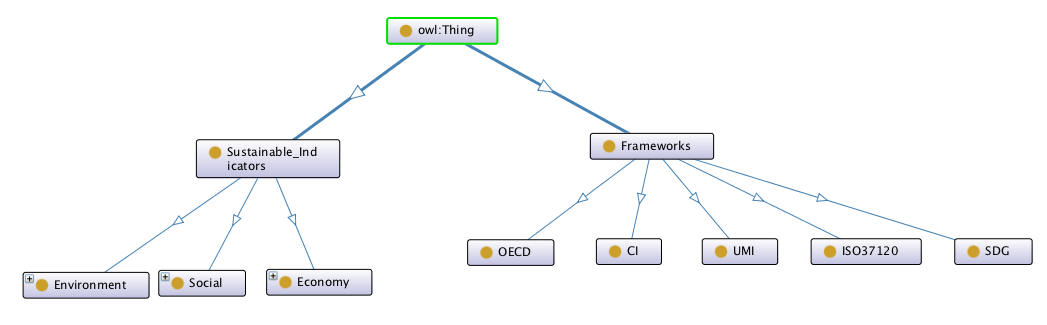
\includegraphics[width=1\textwidth]{figures/ontologyProva.png}
\caption{First two layers of the taxonomy we proposed in this research. The two main classes refer to the 3 pillars of sustainability and to the 5 selected frameworks. }
\label{fig:ontologyProtege}
\end{figure}
Building the ontology is based on an incremental process starting by the identification of the main concepts from the identified approaches dedicated to the three pillars of sustainability and of the indicators of urban systems defined by our frameworks. This process is followed by the extraction of all concepts, properties and relationships from the common meta-model to form the backbone of the ontology. Finally, expanding the extracted concepts to a set of criteria prosecutes to a taxonomy construction. The ontology was built using the Protégé developed by Stanford University \cite{protege}. A graphical illustration of the ontology generated and extracted from Protégé is reported in \figurename~\ref{fig:ontologyProtege}. The ontology is defined by 2 main classes, namely \texttt{Frameworks} and \texttt{Sustainable\_Indicators}. The \texttt{Frameworks} class has 5 subclasses: \texttt{SDG}, \texttt{OECD}, \texttt{ISO37120}, \texttt{UMI}, \texttt{CI} that correspond respectively to \emph{U.S. Cities SDG Index}, \emph{OECD regional and metropolitan database}, \emph{ISO standard 37120}, \emph{Urban Metabolism indicators} and \emph{Cercle Indicators}. The \texttt{Sustainable\_Indicators} class has three main classes defined by the three pillars of sustainability, i.e. \texttt{Economy}, \texttt{Environment}, \texttt{Social}. On. the other hand, for each of the sustainable indicators we created a hierarchical taxonomy for each class. While the \texttt{Frameworks} sub-classes are defined just by a short description of the framework itself, the sub-classes of the \texttt{Sustainable\_Indicators}, such as \texttt{Economy}, \texttt{Social}, \texttt{Environment} have a sub-structure containing the information of the 334 indicators we collected. A comparison of the different frameworks for the different indicators is reported in \figurename~\ref{fig:comparisonFramework} and in Table~\ref{tab:ind}.



\begin{figure}[t!]
\centering
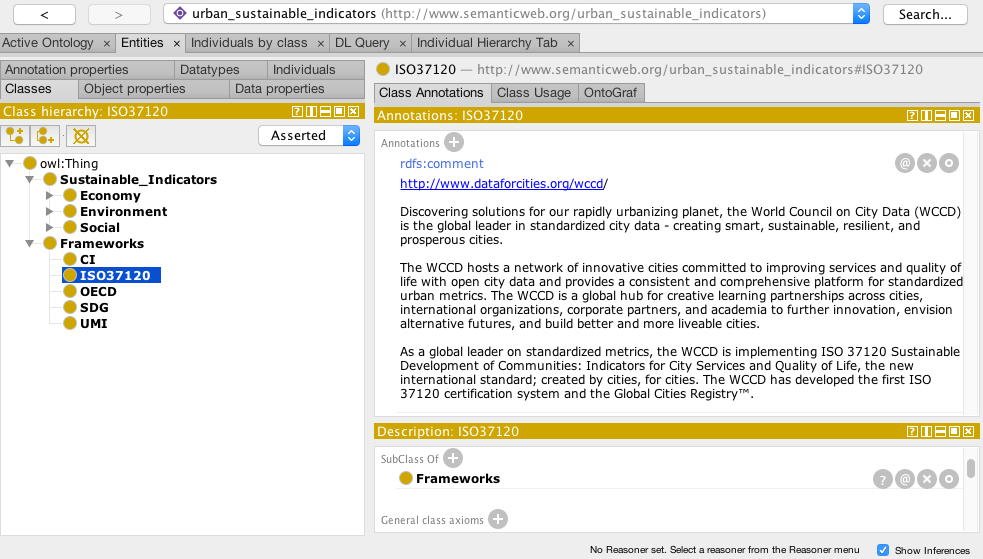
\includegraphics[width=1\textwidth]{figures/ISO.png}
\caption{Description of the  class \texttt{ISO37120} that is subclass of the class \texttt{Frameworks}: for each framework we added a \texttt{comment} about the information of the framework itself.}
\label{fig:ISO}
\end{figure}






\begin{figure}[t!]
\centering
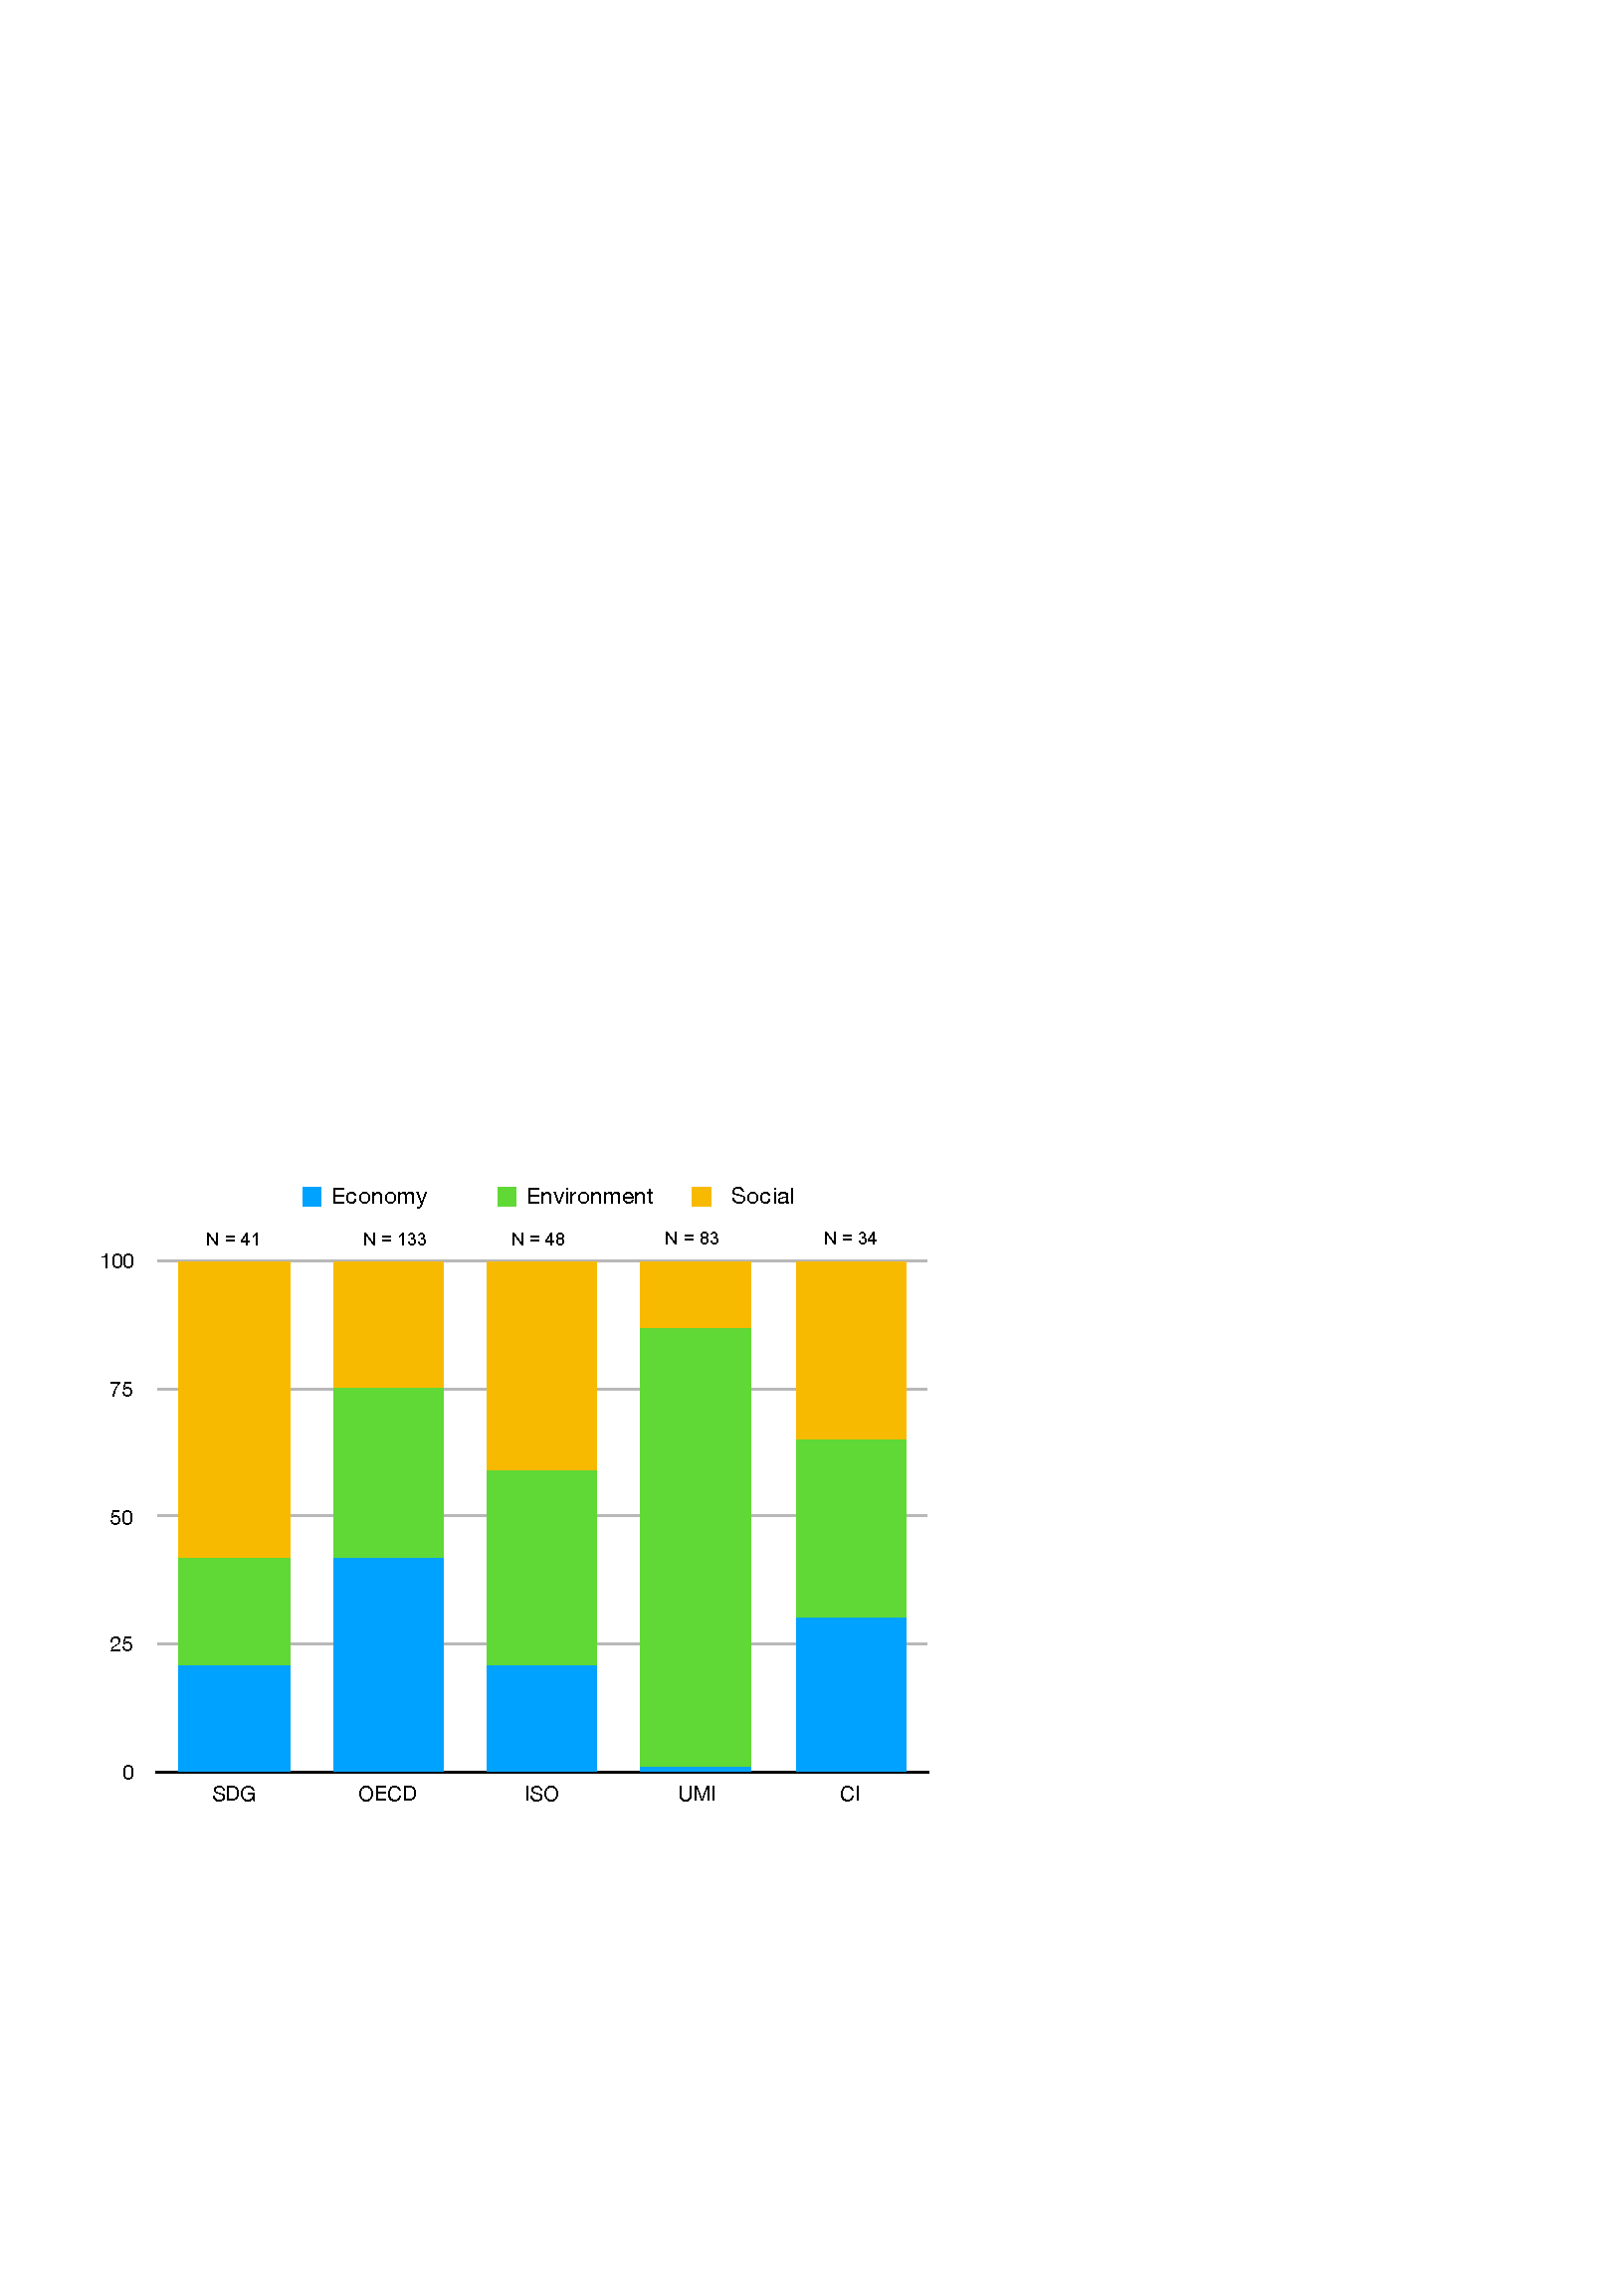
\includegraphics[width=1\textwidth]{figures/chart2.pdf}
\caption{Comparison of the percentage of the different classes for the the different frameworks. As we can see the most equilibrate frameworks is the Cercle Indicators (CI) framework while 
the most unbalanced towards the environmental impact is the Urban Metabolism framework (UMI).}
\label{fig:comparisonFramework}
\end{figure}








\section{Discussion}

This study proposes a new over-arching principle to review the framework from two point of view: i)  the sustainability
pillars: environment, social, and economic and the sustainable indicators from different frameworks:  \emph{U.S. Cities SDG Index}, \emph{OECD regional and metropolitan database}, \emph{ISO standard 37120}, \emph{Urban Metabolism indicators} and \emph{Cercle Indicators}.
While all indicators frameworks are focusing on (urban) sustainability, it becomes evident that they neither address similar aspects of it nor do they address it in a similar way. A key learning point
emerging from the process is that choice of indicators for comparing different cities is a critical
issue both for the efficacy of a stakeholder-driven approach and for the objectives and indicators chosen. The definition of Sustainable Assessment based on the three pillars of sustainability means that an equilibrate approach should take into account in equal distribution all the the three aspects. In \figurename~\ref{fig:comparisonFramework} we show the percentage of the number of indicators under the three classes of sustainability for the different frameworks. We can notice that the most \emph{equiliabrate} framework is given by the Cercle Indicators frameworks where the the three pillars are equally distributed (see Table~\ref{tab:ind}). By our analysis emerges the fact that the ISO 37120  is well distributed and it is the framework with the largest number of indicators, i.e. 133 (see \ref{tab:numberIndicators}). The SDG, OECD and UMI frameworks could be utilized for a sustainable assessment more focused respectively on Social, Economy and Environment (Energy) aspects.


The unique indicator that is present in all the 5 frameworks is \emph{GDP per capita} while some indicators such  unemployment rate, urbanized area, green area are common to numerous indicator frameworks yet their expression can hinder comparability between frameworks or case studies. For instance, the ISO 37120 standard accounts energy use with 3 main indicators: total residential electrical energy use per capita, energy consumption of public buildings per year and total electrical energy use per capita. UMI, accounts energy use (from different sources) in tons and excludes electricity use. In \cite{kennedy2014developing}, the authors distinguish energy use in stationary and mobile and then further disaggregates by fuel type. In addition, it adds the sectoral use of energy (residential, commercial, industrial and transportation. By disaggregating their indicator framework as much as possible, \cite{kennedy2014developing} enhances comparability with other frameworks. Each main subclasses (Economy, Environment and Social) are discussed in the following subsections.

\begin{table}[htb!]
\centering
\begin{tabular}{|l||*{5}{c|}}\hline
\backslashbox{Indicators}{Frameworks}
&\makebox[3em]{SDG}&\makebox[3em]{OECD}&\makebox[3em]{ISO}&\makebox[3em]{UMI}&\makebox[3em]{CI}\\\hline\hline
\textbf{Economy:} &&&&&\\\hline
\text{1) GDP per capita} &$\bigtriangleup$ &$\bullet$ &$\bullet$ &$\bullet$ &$\bullet$\\\hline
\text{2) Unemployment Rate } &$\bullet$ &$\bigtriangleup$ &$\bullet$ & &$\bullet$\\\hline
\text{3) Patent Application} &$\bullet$ &$\bullet$ &&&\\\hline
\textbf{Environment:} &&&&&\\\hline
\text{4) PM 2.5 } &$\bullet$ &$\bullet$ &$\bigtriangleup$ & &\\\hline
\text{5) $CO_2$ per  capita} &$\bigtriangleup$ &$\bullet$ & & &$\bullet$\\\hline
\text{6) Urbanized Area } & &$\bullet$ &$\bullet$ &$\bullet$ &$\bigtriangleup$\\\hline
\text{7) Green Area } &$\bigtriangleup$ &$\bigtriangleup$ &$\bigtriangleup$ &$\bullet$ & \\\hline
\textbf{Social:} &&&&&\\\hline
\text{8) Violent Crimes} &$\bullet$ & &$\bullet$ & &$\bullet$\\\hline
\text{9) Internet Connections} &$\bullet$ & &$\bigtriangleup$ &$\bigtriangleup$ &\\\hline
\text{10) Population Density} & &$\bullet$ &$\bullet$ &$\bigtriangleup$ &\\\hline
\end{tabular}
\caption{\label{tab:ind_cons} The most consistent indicators among the different frameworks: points refer to the exact same indicator while triangles refer to values that can be extracted from the dataset. }
\end{table}


\subsection{Economy}
The indicators under the \texttt{Economy} class were divided according to the following subclasses: Employment, GDP, Labor,  Patent and Others. Table~\ref{tab:ind} represents the economical indicators amount (63 in total) and distribution by frameworks. The most representative framework for a economical analysis would be the OECD with the $42\%$ of indicators that fit into the economy class.  The OECD framework includes 15 indicators, which are equally distributed through our sections: moreover all the indicators in the dataset can be well classified and there are not indicators in the \texttt{Other} subclass.
The Urban Metabolism Indicators framework (UMI) has only 1 indicator in total, which means that we probably won't use this framework for economical sustainability assessment.  

\subsection{Environment}
The Environment indicators subclasses are Air, Climate, Energy, Land, Materials, Waste, Water and Others (see Table~\ref{tab:ind}) . The Urban Metabolism Indicators framework (UMI) has $71$ indicators in total representing the $85\%$ of the total dataset. Most of the data relates to the Energy sector with $46$ indicators in for energy sustainability assessment. In the UMI dataset we were not able to detect indicators characterizing air quality or air pollution. In the same time, it was possible to find a subclass for all the indicators. In fact the subclass ``Others'' results empty: it implies that the chosen environmental subclasses completely satisfy the UMI framework. The environmental indicators represent more the $30\%$ of the ISO, UMI and CI frameworks while only the $20
\%$ for the OECD dataset. 


\subsection{Social}
Crime, Deaths, Education, Health, ICT, Mobility, Population, Poverty, Quality Of Service and Others are the subclasses of the last pillar of Sustainable Indicators.
Table \ref{tab:ind} gives a detailed representation of social indicators in each framework. For the Social class we collected 115 indicators in total. In this context, the SDF framework seems to be the most representative framework for an urban sustainability assessment focused more on the social perspective. 
The U.S. Cities SDG Index framework consist of 28 indicators in the Social class, which were spread almost through all subclasses, except ICT and Population.




\section{Conclusions}

% \section{Similarities and dissimilarities of the indicators}
% 
 



% \subsection{Linkages between datasets}
% There are some clear linkages between the indicator frameworks of the ISO 37120 and the Urban Metabolism. In fact, there was some collaboration between the two parties to develop the ISO 37120.
% Some indicators such energy use, water use, GHG emissions are common to numerous indicator frameworks yet their expression can hinder comparability between frameworks or case studies. For instance, the ISO 37120 standard accounts energy use with 3 main indicators: total residential electrical energy use per capita, energy consumption of public buildings per year and total electrical energy use per capita. EW-MFA, accounts energy use (from different sources) in tons and excludes electricity use. In \cite{kennedy2014developing}, the authors distinguish energy use in stationary and mobile and then further disaggregates by fuel type. In addition, it adds the sectoral use of energy (residential, commercial, industrial and transportation. By disaggregating their indicator framework as much as possible, \cite{kennedy2014developing} enhances comparability with other frameworks.
 
% As these two frameworks come from and are used by academics there are perpetual enhancements. The rest of the indicator framework remain more set in time which represents a certain risk of still being adopted by practitioners on the long run as new sustainability-related concepts appear in the landscape, such as resilience, circular economy, smart cities, etc.
% EW-MFA, is perhaps the only indicator framework that does not explicitly proposes to measure the state of social and economic dimensions of cities (although material flows, their consumption and production are intrinsically connected with these dimensions). In addition, this framework aggregates different challenges as one aggregate metric which are tons. In other frameworks, flows (of energy, materials, water, GHG emissions, etc.) are further disaggregated offering the opportunity to lay out different sustainability challenges simultaneously without any prior focus. The role of the utilities from the Urban Metabolism contains some similar elements  than the ISO 37120.

\section*{Bibliography}

\bibliographystyle{model1-num-names}
\bibliography{sample.bib}

%% Authors are advised to submit their bibtex database files. They are
%% requested to list a bibtex style file in the manuscript if they do
%% not want to use model1-num-names.bst.

%% References without bibTeX database:

% \begin{thebibliography}{00}

%% \bibitem must have the following form:
%%   \bibitem{key}...
%%

% \bibitem{}

% \end{thebibliography}
\section*{Appendix}

\begin{table}[htb!]
\centering
\begin{tabular}{|l||*{5}{c|}}\hline
\backslashbox{Categories}{Frameworks}
&\makebox[3em]{SDG}&\makebox[3em]{OECD}&\makebox[3em]{ISO}&\makebox[3em]{UMI}&\makebox[3em]{CI}\\\hline\hline
\textbf{Economy:} &&&&&\\\hline
\text{1) Employment} &1&5&5&--&1\\\hline
\text{2) GDP} &1&3&4&1&1\\\hline
\text{3) Labor} &--&4&4&--&2\\\hline
\text{4) Patent} &1&3&1&--&--\\\hline
\text{5) Others} &7&--&13&--&6\\\hline
\textbf{Total} & 10 & 15 & 27 & 1 & 10 \\ 
\textbf{Percentage}  & $21\%$ & $ 42\%$ & $21\%$  & $1\%$ & $30\%$ \\
\hline \hline 
\textbf{Environment:} &&&&&\\\hline
\text{1) Air} &3&4&7&--&1\\\hline
\text{2) Climate} &--&--&3&4&1\\\hline
\text{3) Energy} &1&--&7&46&2\\\hline
\text{4) Land} &4&8&9&3&3\\\hline
\text{5) Materials} &--&--&--&4&2\\\hline
\text{6) Waste} &--&--&15&6&--\\\hline
\text{7) Water} &1&--&6&8&2\\\hline
\text{8) Others} &1&--&4&--&1\\\hline
\textbf{Total} & 10 & 12 & 51 & 71 & 12 \\
\textbf{Percentage} & $21\%$ & $33\%$ & $38\%$  & $86\%$ & $35\%$\\\hline\hline
\textbf{Social:} &&&&&\\\hline
\text{1) Crime} &4&--&3&--&1\\\hline
\text{2) Deaths} &3&--&4&--&1\\\hline
\text{3) Education} &4&--&7&--&1\\\hline
\text{4) Health} &7&--&2&--&1\\\hline
\text{5) ICT} &--&--&--&3&--\\\hline
\text{6) Mobility} &3&--&7&--&1\\\hline
\text{7) Population} &--&7&15&1&--\\\hline
\text{8) Poverty} &2&--&--&--&--\\\hline
\text{9) Quality Of Service} &1&--&1&7&1\\\hline
\text{10) Others} &4&2&16&--&6\\\hline
\textbf{Total} &28&9&55&11&12\\
\textbf{Percentage}  & $58 \%$ & $ 25\%$ & $41\%$  & $13\%$ & $35\%$ \\
\hline
\end{tabular}
\caption{\label{tab:ind} The amount and the percentage of indicators for the different the Sustainability subclasses: Economy, Environment and Social.}
\end{table}

\end{document}

%%
%% End of file `elsarticle-template-1-num.tex'.